%%%%%%%% ICML 2018 EXAMPLE LATEX SUBMISSION FILE %%%%%%%%%%%%%%%%%

\documentclass{article}

% Recommended, but optional, packages for figures and better typesetting:
\usepackage{microtype}
\usepackage{graphicx}
\usepackage{subfigure}
\usepackage{booktabs} % for professional tables

% hyperref makes hyperlinks in the resulting PDF.
% If your build breaks (sometimes temporarily if a hyperlink spans a page)
% please comment out the following usepackage line and replace
% \usepackage{icml2018} with \usepackage[nohyperref]{icml2018} above.
\usepackage{hyperref}

% Attempt to make hyperref and algorithmic work together better:
\newcommand{\theHalgorithm}{\arabic{algorithm}}

% Use the following line for the initial blind version submitted for review:
% \usepackage{icml2018}

% If accepted, instead use the following line for the camera-ready submission:
\usepackage[accepted]{icml2018}

% The \icmltitle you define below is probably too long as a header.
% Therefore, a short form for the running title is supplied here:
\icmltitlerunning{MLDL 2018 Fall - Final Project Report}

\begin{document}

\twocolumn[
\icmltitle{MLDL 2018 Fall - Final Project - SqueezeLSTM}

% It is OKAY to include author information, even for blind
% submissions: the style file will automatically remove it for you
% unless you've provided the [accepted] option to the icml2018
% package.

% List of affiliations: The first argument should be a (short)
% identifier you will use later to specify author affiliations
% Academic affiliations should list Department, University, City, Region, Country
% Industry affiliations should list Company, City, Region, Country

% You can specify symbols, otherwise they are numbered in order.
% Ideally, you should not use this facility. Affiliations will be numbered
% in order of appearance and this is the preferred way.
\icmlsetsymbol{equal}{*}

\begin{icmlauthorlist}
\icmlauthor{Jabin Koo (20155009)}{gist}
\icmlauthor{Jinwoo Nam (20155064)}{gist}
\icmlauthor{Junoh Lee (20155134)}{gist}
\end{icmlauthorlist}

\icmlaffiliation{gist}{GIST, South Korea}
% \icmlaffiliation{goo}{Googol ShallowMind, New London, Michigan, USA}
% \icmlaffiliation{ed}{School of Computation, University of Edenborrow, Edenborrow, United Kingdom}

\icmlcorrespondingauthor{Jonghyun Choi}{jhc@gist.ac.kr}
% \icmlcorrespondingauthor{Eee Pppp}{ep@eden.co.uk}

% You may provide any keywords that you
% find helpful for describing your paper; these are used to populate
% the "keywords" metadata in the PDF but will not be shown in the document
\icmlkeywords{Machine Learning, ICML}

\vskip 0.3in
]

% this must go after the closing bracket ] following \twocolumn[ ...

% This command actually creates the footnote in the first column
% listing the affiliations and the copyright notice.
% The command takes one argument, which is text to display at the start of the footnote.
% The \icmlEqualContribution command is standard text for equal contribution.
% Remove it (just {}) if you do not need this facility.

\printAffiliationsAndNotice{}  % leave blank if no need to mention equal contribution
% \printAffiliationsAndNotice{\icmlEqualContribution} % otherwise use the standard text.

% \begin{abstract}
% awesome abstract
% \end{abstract}

\section*{Proposal}
\setlength\parindent{8pt}
In computer vision area with Convolutional Neural Network(CNN), it is quite common that replacing 5x5 convolution kernels by two of 3x3 kernels to reduce the computational cost\cite{Inception}. However for RNN-like cells, there are few or none of such things due to the complexity of the cell.

In this proposal, we will introduce a Recurrent Neural Network(RNN) structure that is efficient in the aspect of number of parameters. RNN(and its variants) is a basic neural network cell that works very well on sequential inputs so widely adopted for Natural Language Processing(NLP), video processing etc. It is composed of hidden layer and output layer. Hidden layer is a layer that feed RNN status to next RNN and fed by previous RNN, and output layer is a layer that gives actual output of network.

Improving the performance of the RNN cell, one common choice is increasing the number of the hidden parameters. However, this approach is not possible for many users. Making hidden layer requires huge amount of memory and computational power but most RNN users are not affordable for it. Also, making RNN hidden layer bigger is risky because it tends to overfit when we increase the size of hidden layer. So our object is to find a novel approach to reduce those cost while keeping its performance as much as possible.

There are not that much works that deals with this problem directly. However, inspired by the technique explained above(replacing 5x5 kernel by two of 3x3), we came up with a brand new approach that factorizing a huge RNN cell into small cells. One approach for this is explained on Figure \ref{fig:RNNcell1}. The figure shows the factorized RNN cells with smaller hidden layer size. Initially, the input only goes to cell 1 and updates the hidden state of the cell. For following input, we use the hidden state of the cell1 to determine which cell to use to process the input. We then repeat this until the end of the input sequence.
\begin{figure}
  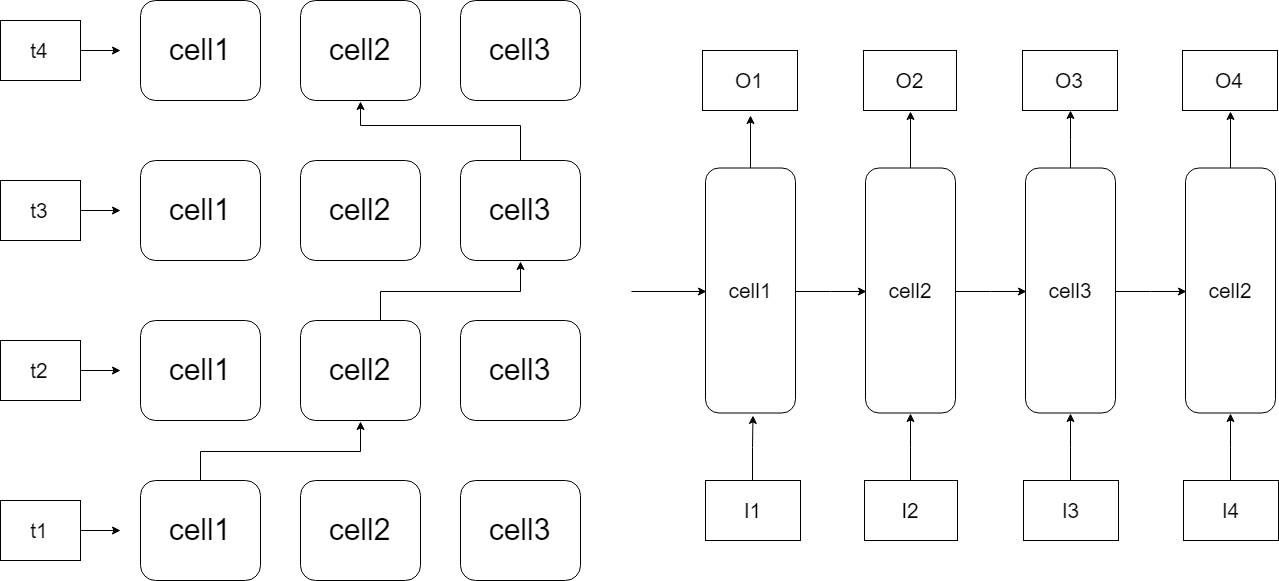
\includegraphics[width=\linewidth]{pictures/RNNfig1.png}
  \caption{One kind of example figure for factorized RNN cells.}
  \label{fig:RNNcell1}
\end{figure}
$$h_t = \sigma(W_hx_t+U_hh_{t-1}+b_h)\label{Elman}$$
$$y_t = \sigma_y(W_yh_t+b_y)$$
\cite{Elman90}

From Elman network which is fully recurrent network, can represent equation \ref{Elman}. Suppose size of hidden layer and size of input size as $n$ and $k$ each. To get hidden state of Elman network we need $n^2+nk+n$ parameters. Let us factorize the cell into 3 cells. Than hidden size become $\frac{n}{3}$ in this network we need $3(\frac{n}{3}^2+\frac{n}{3}k+\frac{n}{3}) = \frac{n^2}{3}+nk+n$. This consider total parameter in RNN cells. In real computation we do not update whole parameter in RNN cells. Thus, in real computation, we can expect less cost.




\section{Intro}
Your intro goes here.

\section{Related Work}
Summarize what you've read that are relevant to your approach.


\section{Approach}
Describe your approach in detail.

\section{Datasets}
Describe the dataset you've used for the project.

\section{Experiments}
Describe the experimental results in detail.

\section{Conclusion}
What do you conclude?


% In the unusual situation where you want a paper to appear in the
% references without citing it in the main text, use \nocite

\bibliography{./sections/mybib.bib}
\bibliographystyle{icml2018}


\end{document}


% This document was modified from the file originally made available by
% Pat Langley and Andrea Danyluk for ICML-2K. This version was created
% by Iain Murray in 2018. It was modified from a version from Dan Roy in
% 2017, which was based on a version from Lise Getoor and Tobias
% Scheffer, which was slightly modified from the 2010 version by
% Thorsten Joachims & Johannes Fuernkranz, slightly modified from the
% 2009 version by Kiri Wagstaff and Sam Roweis's 2008 version, which is
% slightly modified from Prasad Tadepalli's 2007 version which is a
% lightly changed version of the previous year's version by Andrew
% Moore, which was in turn edited from those of Kristian Kersting and
% Codrina Lauth. Alex Smola contributed to the algorithmic style files.
